\section{The BYTE-90 AI Interactive Designer Toy}

The BYTE-90, developed by ALXV Labs, is a compact interactive device that blends elements of retro computing aesthetics with modern embedded system capabilities \cite{byte90_alxv}. Designed to resemble a miniature vintage computer, it serves not as a traditional computing tool but as a programmable desk companion. Its purpose lies in creating an engaging user experience through expressive animations, motion-based interaction, and connectivity features, making it both a collectible item and a development platform for enthusiasts.

\begin{figure}[ht]
    \centering
    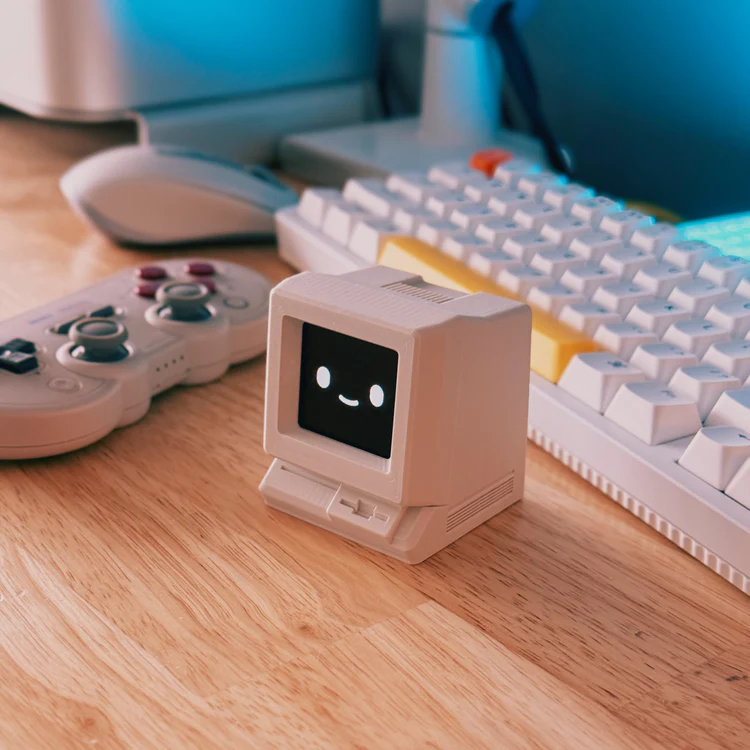
\includegraphics[width=0.4\textwidth]{related-work/image/byte90_complete_product.png}
    \caption{BYTE-90 AI Interactive Designer Toy \cite{byte90_alxv}.}
    \label{fig:byte90_complete_product}
\end{figure}

At its core, the BYTE-90 is powered by an ESP32-S3 microcontroller \cite{byte90_fullproduct}, a widely used chip in Internet of Things (IoT) applications due to its integrated WiFi and Bluetooth capabilities \cite{esp32s3_datasheet}. This allows the device to communicate wirelessly with other units and external systems. The device is also equipped with a low power 128×128 resolution OLED display, which is used to render a variety of animated expressions and visual feedback with 65K RGB colors \cite{byte90_fullproduct}. These animations are central to the device's appeal, as they simulate emotional states or reactions based on user input or environmental changes.

\begin{figure}[ht]
    \centering
    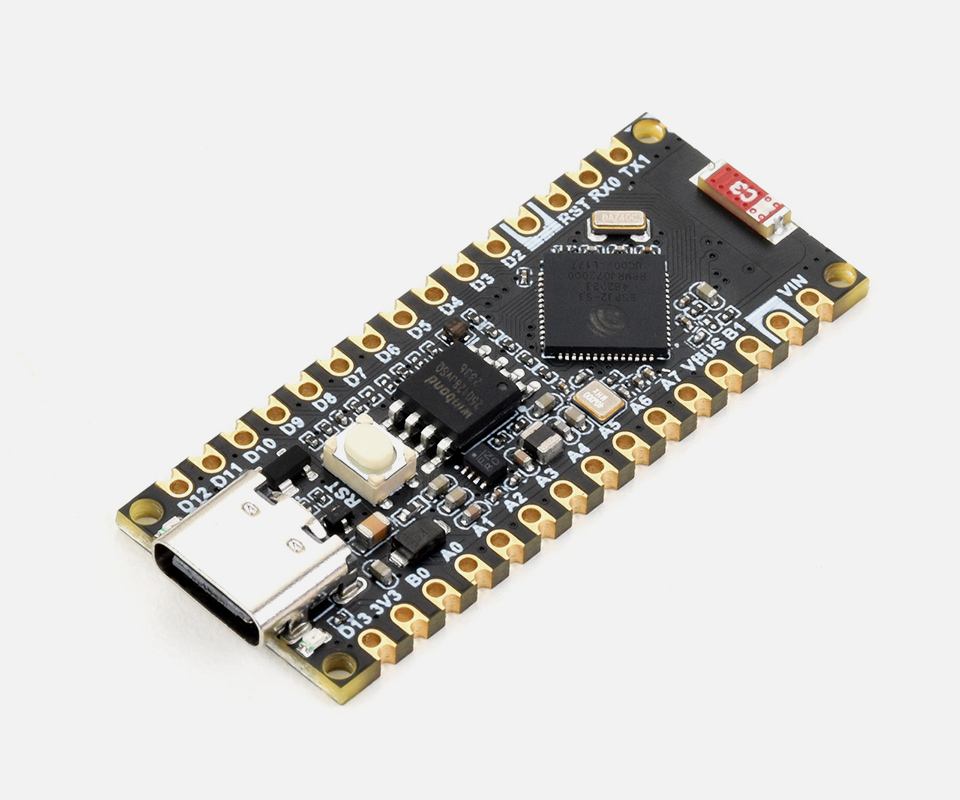
\includegraphics[width=0.4\textwidth]{related-work/image/esp32s3_product.png}
    \caption{ESP32-S3 microcontroller used in the BYTE-90 \cite{esp32s3_product}.}
    \label{fig:esp32s3_product}
\end{figure}

Physically, the BYTE-90 is constructed with 3D-printed PLA bioplastic \cite{byte90_housing}. This choice of material and manufacturing method reflects a focus on accessibility and customization, as users and developers can potentially modify or reproduce parts of the device.

\begin{figure}[ht]
    \centering
    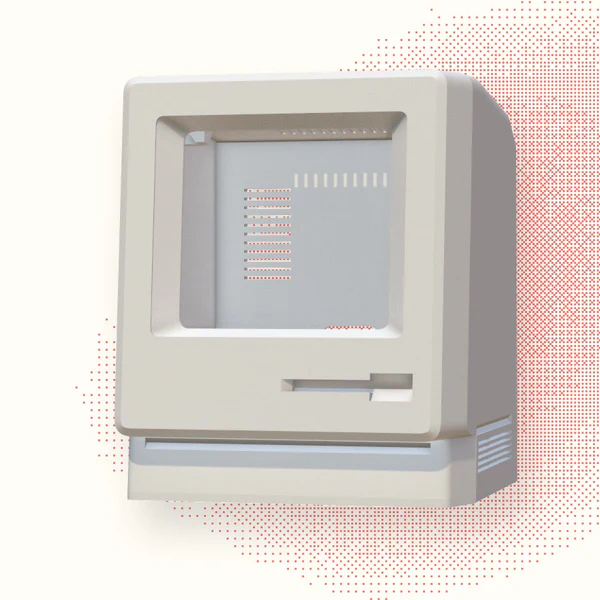
\includegraphics[width=0.4\textwidth]{related-work/image/byte90_housing.png}
    \caption{BYTE-90 AI Interactive Designer Toy Housing \cite{byte90_housing}.}
    \label{fig:byte90_housing}
\end{figure}

\begin{sloppypar}
    From a software perspective, ALXV Labs provides open-source firmware \cite{byte90_firmware}, allowing developers to create their own animations, interaction logic, or communication protocols. This makes it a valuable platform for learning embedded programming, sensor integration, and real-time system design. Users can extend the device's capabilities beyond its default behavior, tailoring it to specific applications or creative ideas.
\end{sloppypar}

In summary, the BYTE-90 represents a convergence of embedded technology and interactive design. It is not intended to compete with conventional computing devices, but rather to offer a unique blend of functionality and personality. For students and developers, it serves as both an inspiration and a reference model for projects that aim to combine hardware, software, and user experience into a cohesive and engaging system.